% =====================================================================
%  Modélisation et commande d'une chaîne éolienne PMSG 2 MW à attaque
%  directe (back-to-back) : commande plate + passive + ANN adaptatif
%  Compilation : pdflatex modelisation_PMSG.tex   (deux fois)
% =====================================================================
\pdfminorversion=4
\pdfobjcompresslevel=0
\documentclass[11pt,a4paper]{article}
\usepackage[utf8]{inputenc}
\usepackage[T1]{fontenc}
\usepackage[french]{babel}
\usepackage{lmodern}
\usepackage[margin=2.3cm]{geometry}
\usepackage{amsmath,amssymb,amsthm,bm}
\usepackage{graphicx}
\usepackage{booktabs,array,multirow}
\usepackage{siunitx}
\usepackage{xcolor}
\usepackage{caption}
\usepackage[hidelinks]{hyperref}
\sisetup{output-decimal-marker={,}, group-separator={\,}}
\graphicspath{{figures/}}

\newtheorem{proposition}{Proposition}
\newtheorem{theoreme}{Théorème}
\theoremstyle{remark}
\newtheorem{remarque}{Remarque}

\newcommand{\Jm}{\mathbf{J}}            % matrice antisymétrique
\newcommand{\vect}[1]{\bm{#1}}
\newcommand{\eq}{\vect{e}_q}

\title{\textbf{Modélisation et commande d'une chaîne éolienne PMSG de \SI{2}{MW}\\
à attaque directe (convertisseur \emph{back-to-back})}\\[2mm]
\large Commande par platitude, commande passive et compensation adaptative par réseau de neurones}
\author{Said Regani\\ \small Laboratoire L2EI, Université de Jijel}
\date{\today}

\begin{document}
\maketitle

\begin{abstract}
Ce document rassemble la modélisation complète d'une chaîne de conversion éolienne de \SI{2}{MW}
à génératrice synchrone à aimants permanents (PMSG) à attaque directe, raccordée au réseau
\SI{690}{V}/\SI{50}{Hz} par un redresseur MLI, un bus continu, un onduleur MLI et un filtre $L$.
Il présente ensuite la commande proposée : commande par platitude pour les boucles externes
(vitesse de rotation pour la MPPT et énergie du bus continu), commande passive (PBC) pour les boucles
de courant des deux convertisseurs, et compensation adaptative par un réseau de neurones 6-10-2
($u=u_N+u_{AI}$) qui ne modifie pas les gains nominaux. Les résultats de simulation en
conditions nominales et en présence d'incertitudes paramétriques sont donnés.
\end{abstract}

\tableofcontents
\newpage

% =====================================================================
\section{Description du système}
% =====================================================================
La chaîne étudiée (figure~\ref{fig:schema}) comprend :
\begin{itemize}
  \item une turbine tripale de rayon $R=\SI{40}{m}$, de vitesse nominale $\Omega_n=\SI{2,23}{rad/s}$ ;
  \item une PMSG à pôles lisses entraînée directement, sans multiplicateur (attaque directe) ;
  \item un convertisseur \emph{back-to-back} : redresseur MLI côté machine (MSC), bus continu
        de capacité $C$, onduleur MLI côté réseau (GSC) ;
  \item un filtre $L$ ($R_f$, $L_f$) et le réseau \SI{690}{V}, \SI{50}{Hz}.
\end{itemize}

\begin{figure}[h]
  \centering
  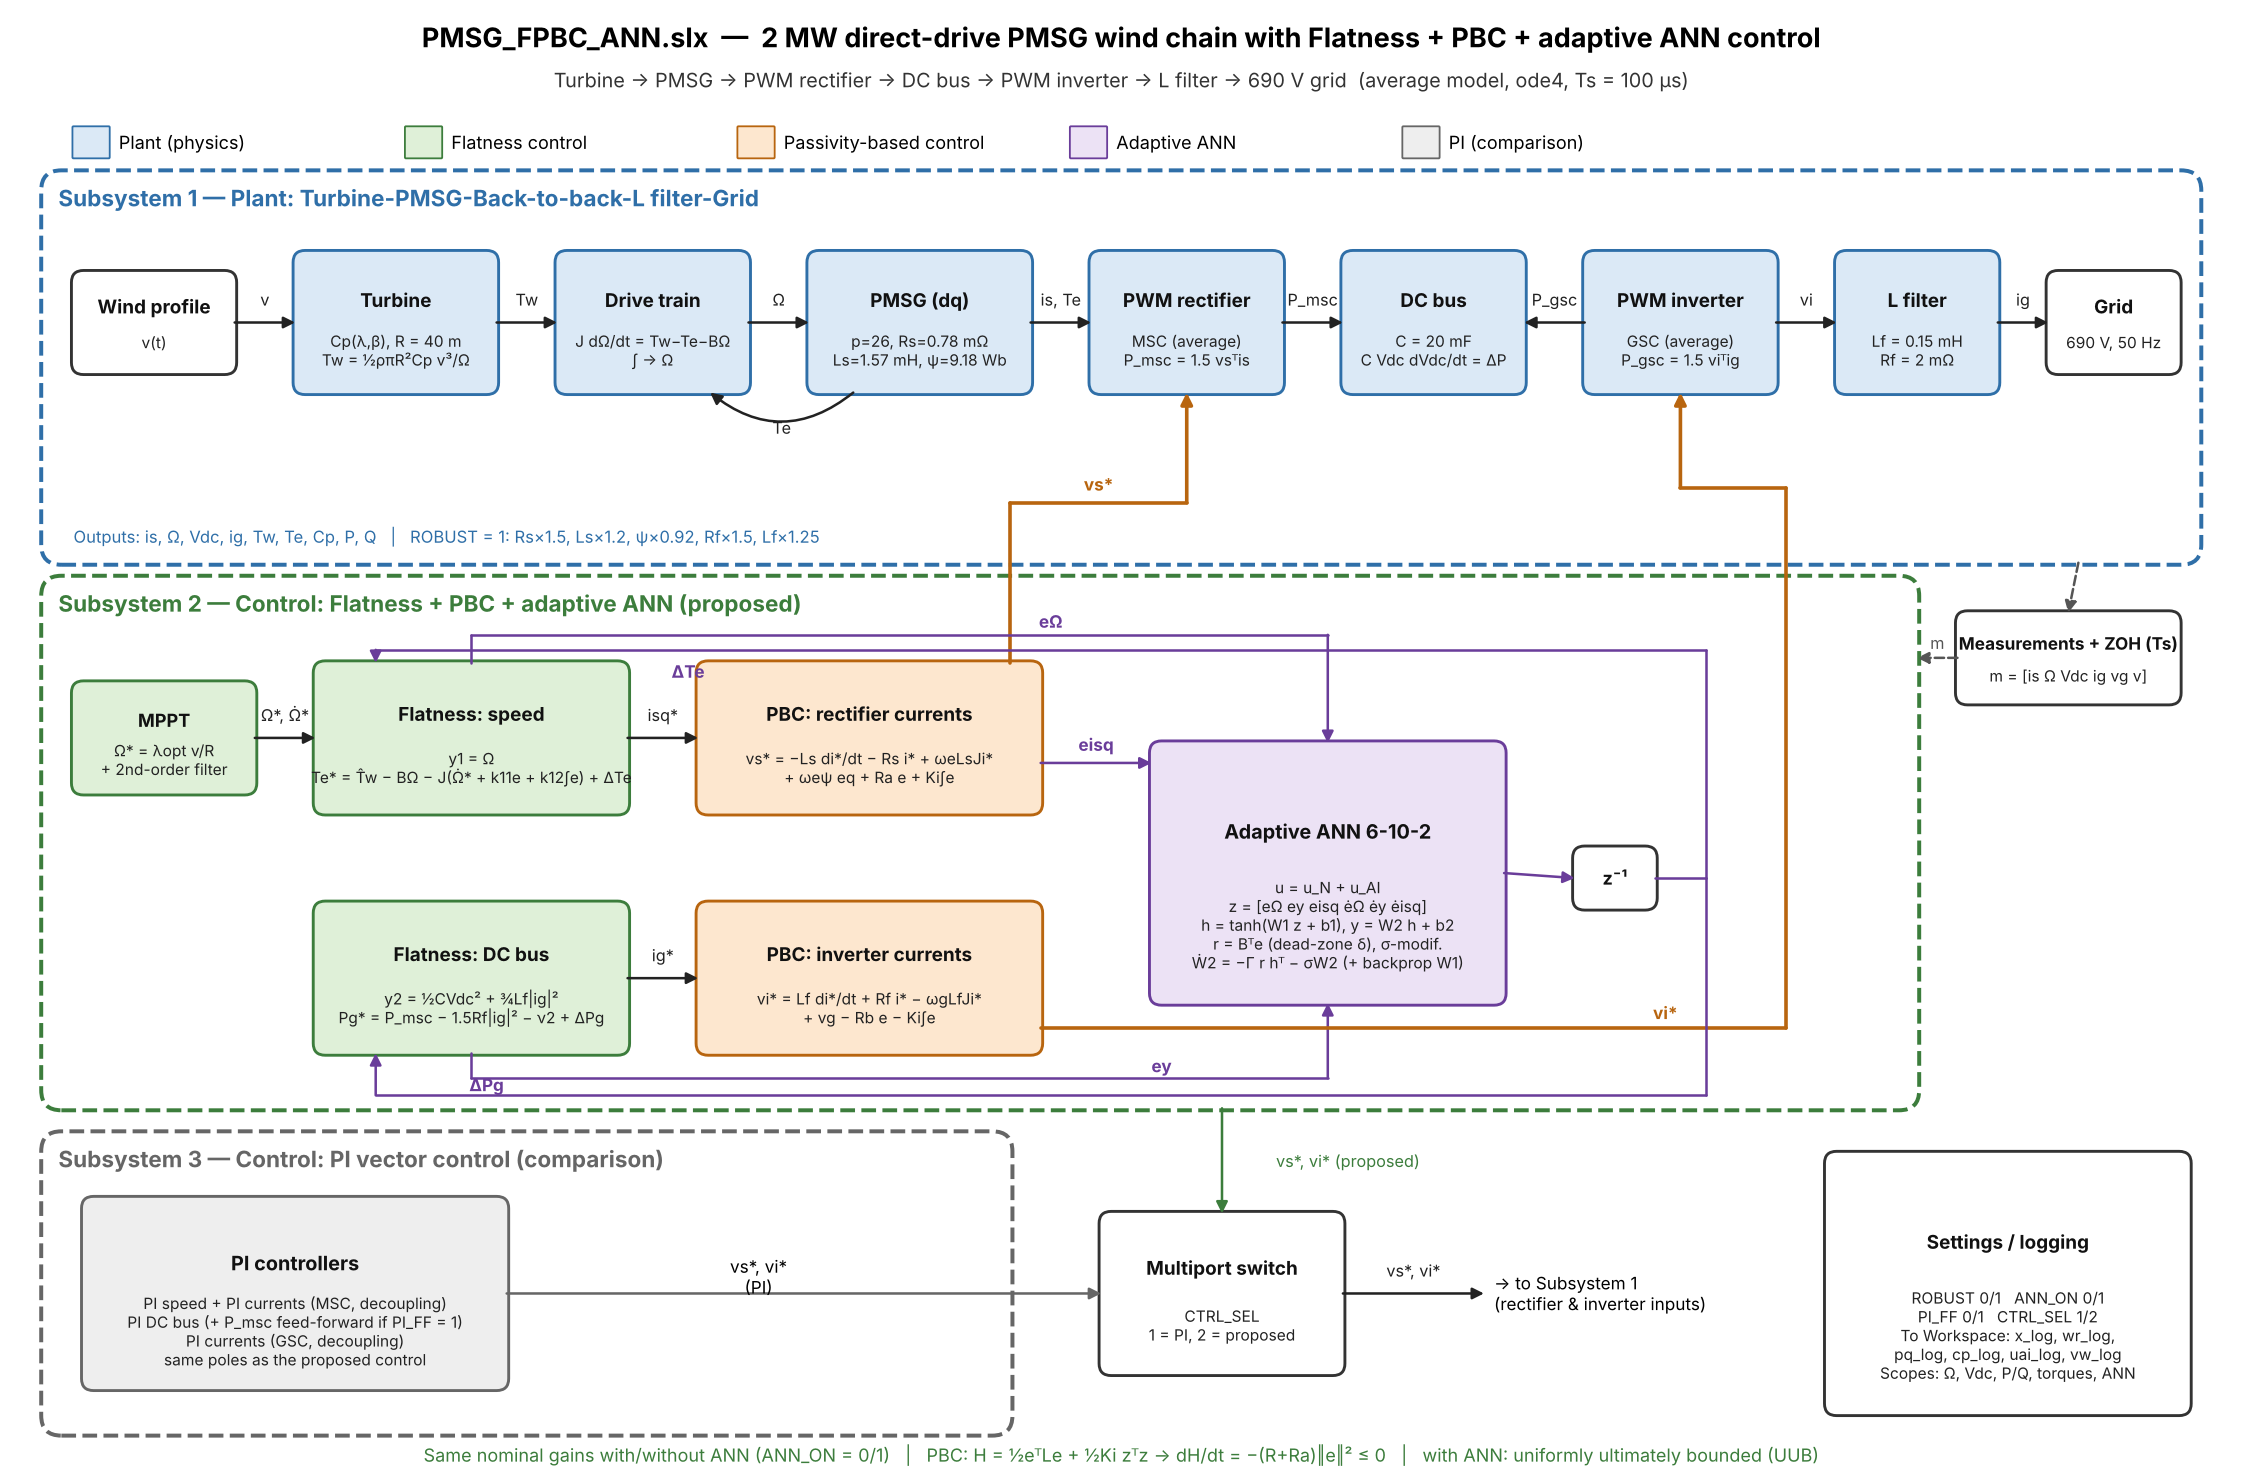
\includegraphics[width=\textwidth]{simulink_diagram.png}
  \caption{Structure complète du système et de la commande (modèle Simulink \texttt{PMSG\_FPBC\_ANN}).}
  \label{fig:schema}
\end{figure}

% =====================================================================
\section{Modélisation de la chaîne}
% =====================================================================

\subsection{Profil de vent}
On utilise le même profil de vent turbulent que dans~\cite{regani} (équation (80)) :
\begin{equation}
  v(t) = V_{mean} + \sum_{k=1}^{3} A_k \sin(2\pi f_k t) + v_{turb}(t),
  \label{eq:vent}
\end{equation}
où $V_{mean}=\SI{8}{m/s}$ est la vitesse moyenne, $A_k$ et $f_k$ l'amplitude et la fréquence de la
$k$-ième composante harmonique, et $v_{turb}(t)$ une composante stochastique gaussienne lissée qui
représente la turbulence. Les valeurs retenues (tableau~\ref{tab:vent}) reproduisent la figure~3
de~\cite{regani} à \SI{0,02}{m/s} près : le vent part de \SI{8}{m/s}, atteint \SI{9}{m/s} vers
$t=\SI{2}{s}$, redescend à \SI{8,6}{m/s} vers $t=\SI{4,2}{s}$, puis monte à \SI{10}{m/s} vers
$t=\SI{7,7}{s}$.

\begin{table}[h]
\centering
\caption{Paramètres du profil de vent (\ref{eq:vent}).}
\label{tab:vent}
\begin{tabular}{lccc}
\toprule
& $k=1$ & $k=2$ & $k=3$\\
\midrule
$A_k$ [\si{m/s}] & 1,5 & 0,2 & 0,3\\
$f_k$ [\si{Hz}] & 0,03 & 0,16 & 0,17\\
\midrule
\multicolumn{4}{l}{$v_{turb}$ : bruit gaussien filtré (1\textsuperscript{er} ordre, $\tau=\SI{0,05}{s}$),
écart type \SI{0,01}{m/s}}\\
\bottomrule
\end{tabular}
\end{table}

\subsection{Turbine}
La puissance captée par la turbine et le couple aérodynamique s'écrivent :
\begin{equation}
  P_w = \tfrac12\,\rho\,\pi R^2\,C_p(\lambda,\beta)\,v^3, \qquad
  T_w = \frac{P_w}{\Omega}, \qquad
  \lambda = \frac{\Omega R}{v},
  \label{eq:turbine}
\end{equation}
où $\lambda$ est la vitesse spécifique et $\beta$ l'angle de calage. Le coefficient de puissance
est donné par le modèle de Heier :
\begin{equation}
  C_p(\lambda,\beta) = 0{,}5176\left(\frac{116}{\lambda_i} - 0{,}4\beta - 5\right)e^{-21/\lambda_i}
  + 0{,}0068\,\lambda,
  \qquad
  \frac{1}{\lambda_i} = \frac{1}{\lambda+0{,}08\beta} - \frac{0{,}035}{\beta^3+1}.
\end{equation}
Pour $\beta=0$, le maximum $C_{p,\max}=0{,}48$ est atteint pour $\lambda_{opt}=8{,}1$.

\paragraph{Cohérence des données.} Avec $\Omega_n=\SI{2,23}{rad/s}$ et $\lambda_{opt}=8{,}1$, le vent
nominal vaut $v_n=\Omega_n R/\lambda_{opt}\approx\SI{11}{m/s}$, et
$P_w=\tfrac12\rho\pi R^2\,0{,}48\,v_n^3\approx\SI{1,97}{MW}$, ce qui correspond bien à
$P_n=\SI{2}{MW}$ et à $T_n=P_n/\Omega_n\approx\SI{0,9}{MN.m}$.

\subsection{Arbre de transmission}
L'attaque directe permet un modèle mono-masse :
\begin{equation}
  J\,\frac{d\Omega}{dt} = T_w - T_e - B\,\Omega ,
  \label{eq:arbre}
\end{equation}
où $J$ est l'inertie totale (turbine + génératrice) et $B$ le frottement visqueux.

\subsection{Génératrice synchrone à aimants permanents}
On utilise la transformation de Park (invariance d'amplitude) dans le repère $dq$ lié au rotor,
l'axe $d$ étant aligné sur le flux des aimants. Avec la convention générateur et $L_d=L_q=L_s$ :
\begin{align}
  L_s\frac{di_{sd}}{dt} &= -R_s i_{sd} + \omega_e L_s i_{sq} - v_{sd}, \label{eq:pmsg_d}\\
  L_s\frac{di_{sq}}{dt} &= -R_s i_{sq} - \omega_e L_s i_{sd} + \omega_e\psi_f - v_{sq}, \label{eq:pmsg_q}\\
  T_e &= \tfrac32\,p\,\psi_f\, i_{sq}, \qquad \omega_e = p\,\Omega, \label{eq:couple}
\end{align}
où $p$ est le nombre de paires de pôles et $\psi_f$ le flux des aimants.

\paragraph{Forme vectorielle.} En notant $\vect{i}_s=[i_{sd}\;i_{sq}]^T$,
$\vect{v}_s=[v_{sd}\;v_{sq}]^T$, $\eq=[0\;1]^T$ et
\begin{equation}
  \Jm = \begin{bmatrix} 0 & 1\\ -1 & 0\end{bmatrix} = -\Jm^T ,
\end{equation}
le modèle (\ref{eq:pmsg_d})--(\ref{eq:pmsg_q}) devient
\begin{equation}
  L_s\,\dot{\vect{i}}_s = -R_s\,\vect{i}_s + \omega_e L_s\,\Jm\,\vect{i}_s + \omega_e\psi_f\,\eq - \vect{v}_s .
  \label{eq:pmsg_vect}
\end{equation}
Le terme $\omega_e L_s\Jm\vect{i}_s$ est un couplage \emph{sans travail} :
$\vect{i}_s^T\Jm\,\vect{i}_s=0$. Le bilan d'énergie magnétique
$H_s=\tfrac12 L_s\|\vect{i}_s\|^2$ s'écrit
\begin{equation}
  \dot H_s = -R_s\|\vect{i}_s\|^2 + \omega_e\psi_f\, i_{sq} - \vect{i}_s^T\vect{v}_s ,
\end{equation}
c'est-à-dire : puissance électromécanique reçue $-$ pertes Joule $-$ puissance fournie au redresseur.
C'est cette structure (Euler--Lagrange / Hamiltonienne à ports) qu'exploite la commande passive.

\subsection{Convertisseurs MLI (modèle moyen)}
Les deux convertisseurs sont des ponts à deux niveaux commandés en MLI vectorielle (SVPWM).
Sur une période de découpage, leurs tensions moyennes dans le repère $dq$ sont
\begin{equation}
  \vect{v}_s = \tfrac{V_{dc}}{2}\,\vect{m}_s, \qquad
  \vect{v}_i = \tfrac{V_{dc}}{2}\,\vect{m}_i, \qquad
  \|\vect{m}\| \le \tfrac{2}{\sqrt3}
  \;\;\Longleftrightarrow\;\;
  \|\vect{v}\| \le \frac{V_{dc}}{\sqrt3},
  \label{eq:mli}
\end{equation}
où $\vect{m}$ est le vecteur des indices de modulation. Les convertisseurs étant supposés sans pertes,
les courants côté continu se déduisent de la conservation de la puissance :
\begin{equation}
  P_{msc} = \tfrac32\,\vect{v}_s^T\vect{i}_s = V_{dc}\, i_{dc,msc}, \qquad
  P_{gsc} = \tfrac32\,\vect{v}_i^T\vect{i}_g = V_{dc}\, i_{dc,gsc}.
\end{equation}

\begin{remarque}
Le modèle commuté (ponts à deux niveaux, porteuse triangulaire à \SI{2160}{Hz}, échantillonnage
régulier à double mise à jour) a aussi été simulé. Il sert à vérifier la qualité de l'onde
(THD du courant réseau). Le modèle moyen est utilisé pour la synthèse de la commande.
\end{remarque}

\subsection{Bus continu}
\begin{equation}
  C\,V_{dc}\,\frac{dV_{dc}}{dt} = P_{msc} - P_{gsc}
  \quad\Longleftrightarrow\quad
  \frac{dW_{dc}}{dt} = P_{msc} - P_{gsc}, \qquad W_{dc} = \tfrac12 C V_{dc}^2 .
  \label{eq:bus}
\end{equation}

\subsection{Filtre \texorpdfstring{$L$}{L} et réseau}
Le repère $dq$ côté réseau est orienté sur la tension du réseau (PLL supposée idéale) :
$v_{gd}=V_m=\sqrt{2/3}\,U$, $v_{gq}=0$. Le courant $\vect{i}_g$ va de l'onduleur vers le réseau :
\begin{equation}
  L_f\,\dot{\vect{i}}_g = -R_f\,\vect{i}_g + \omega_g L_f\,\Jm\,\vect{i}_g + \vect{v}_i - \vect{v}_g ,
  \label{eq:filtre}
\end{equation}
et les puissances injectées au réseau valent
\begin{equation}
  P = \tfrac32\,(v_{gd} i_{gd} + v_{gq} i_{gq}) = \tfrac32 V_m i_{gd}, \qquad
  Q = \tfrac32\,(v_{gq} i_{gd} - v_{gd} i_{gq}) = -\tfrac32 V_m i_{gq}.
\end{equation}
Le facteur de puissance unitaire correspond donc à $i_{gq}=0$.

\subsection{Modèle d'état complet}
Avec l'état, les entrées de commande et les perturbations
\begin{equation}
  \vect{x} = [\,i_{sd}\;\; i_{sq}\;\; \Omega\;\; V_{dc}\;\; i_{gd}\;\; i_{gq}\,]^T, \qquad
  \vect{u} = [\,v_{sd}\;\; v_{sq}\;\; v_{id}\;\; v_{iq}\,]^T, \qquad
  \vect{d} = [\,v\;\; v_{gd}\;\; v_{gq}\,]^T,
\end{equation}
la chaîne complète est décrite par le système non linéaire d'ordre 6 :
\begin{equation}
\left\{
\begin{aligned}
  \dot i_{sd} &= \tfrac{1}{L_s}\bigl(-R_s i_{sd} + p\Omega L_s i_{sq} - v_{sd}\bigr)\\
  \dot i_{sq} &= \tfrac{1}{L_s}\bigl(-R_s i_{sq} - p\Omega L_s i_{sd} + p\Omega\psi_f - v_{sq}\bigr)\\
  \dot \Omega &= \tfrac{1}{J}\Bigl(\tfrac{\rho\pi R^2 C_p(\lambda,\beta) v^3}{2\Omega}
                 - \tfrac32 p\psi_f i_{sq} - B\Omega\Bigr)\\
  \dot V_{dc} &= \tfrac{3}{2\,C\,V_{dc}}\bigl(v_{sd}i_{sd} + v_{sq}i_{sq} - v_{id}i_{gd} - v_{iq}i_{gq}\bigr)\\
  \dot i_{gd} &= \tfrac{1}{L_f}\bigl(-R_f i_{gd} + \omega_g L_f i_{gq} + v_{id} - v_{gd}\bigr)\\
  \dot i_{gq} &= \tfrac{1}{L_f}\bigl(-R_f i_{gq} - \omega_g L_f i_{gd} + v_{iq} - v_{gq}\bigr)
\end{aligned}
\right.
\label{eq:modele_complet}
\end{equation}
avec la contrainte $\|\vect{v}_s\|,\|\vect{v}_i\|\le V_{dc}/\sqrt3$.

\subsection{Point de fonctionnement MPPT}
Pour un vent $v_0$ constant, le régime permanent à puissance maximale est :
\begin{equation}
\begin{gathered}
  \Omega_0 = \frac{\lambda_{opt} v_0}{R},\quad
  i_{sd,0}=0,\quad
  i_{sq,0} = \frac{T_w(\Omega_0,v_0) - B\Omega_0}{\tfrac32 p\psi_f},\\
  \vect{v}_{s,0} = \begin{bmatrix} \omega_{e0}L_s i_{sq,0}\\ \omega_{e0}\psi_f - R_s i_{sq,0}\end{bmatrix},\quad
  i_{gd,0} = \frac{P_{msc,0}}{\tfrac32 V_m},\quad i_{gq,0}=0,\quad V_{dc,0}=V_{dc}^*.
\end{gathered}
\end{equation}
Ce point initialise toutes les simulations.

\paragraph{Vérification de la PMSG.} À la fréquence nominale de la machine de~\cite{hasan}
(\SI{9,75}{Hz}), la f.é.m. vaut $E=\psi_f\,\omega_e = 9{,}18\times 2\pi\times 9{,}75\approx\SI{562}{V}$,
soit la tension simple crête du réseau \SI{690}{V} ($\SI{563}{V}$). Au point nominal de la turbine
($\Omega=\SI{2,23}{rad/s}$, $i_{sq}\approx\SI{2,5}{kA}$), la tension du redresseur vaut
$\|\vect{v}_s\|\approx\SI{580}{V} < V_{dc}/\sqrt3 = \SI{693}{V}$.

\subsection{Paramètres}
\begin{table}[h]
\centering
\caption{Paramètres de la chaîne étudiée.}
\label{tab:param}
\begin{tabular}{llll}
\toprule
Grandeur & Symbole & Valeur & Source\\
\midrule
\multicolumn{4}{l}{\emph{Turbine}}\\
Puissance nominale & $P_n$ & \SI{2}{MW} & encadrant ; \cite{hasan}\\
Rayon du rotor & $R$ & \SI{40}{m} & encadrant\\
Vitesse nominale & $\Omega_n$ & \SI{2,23}{rad/s} & encadrant\\
Couple nominal & $T_n$ & \SI{0,897}{MN.m} & $P_n/\Omega_n$\\
Vitesse spécifique optimale & $\lambda_{opt}$ & 8,1 ($C_{p,\max}=0{,}48$) & \cite{hasan}\\
Masse volumique de l'air & $\rho$ & \SI{1,225}{kg/m^3} & --\\
Inertie totale & $J$ & \SI{2,8e6}{kg.m^2} ($H\approx\SI{3,5}{s}$) & hypothèse\\
Frottement & $B$ & \SI{1000}{N.m.s/rad} & hypothèse\\
\midrule
\multicolumn{4}{l}{\emph{PMSG (pôles lisses)}}\\
Paires de pôles & $p$ & 26 & \cite{hasan}, Tab.~I\\
Résistance statorique & $R_s$ & \SI{0,78}{m\ohm} & \cite{hasan}, Tab.~I\\
Inductance synchrone & $L_s=L_d=L_q$ & \SI{1,57}{mH} & \cite{hasan}, Tab.~I\\
Flux des aimants & $\psi_f$ & \SI{9,18}{Wb} & \cite{hasan}, Tab.~I\\
\midrule
\multicolumn{4}{l}{\emph{Bus continu, filtre, réseau}}\\
Capacité & $C$ & \SI{20}{mF} & \cite{hasan}, Tab.~I\\
Tension de référence & $V_{dc}^*$ & \SI{1200}{V} & \cite{hasan}, Fig.~12\\
Inductance du filtre & $L_f$ & \SI{0,15}{mH} & \cite{hasan}, Fig.~4a\\
Résistance du filtre & $R_f$ & \SI{2}{m\ohm} & hypothèse\\
Réseau & $U$, $f$ & \SI{690}{V}, \SI{50}{Hz} & \cite{hasan}, Tab.~I\\
Fréquence de découpage & $f_{sw}$ & \SI{2160}{Hz} & \cite{hasan}, §IV\\
\bottomrule
\end{tabular}
\end{table}

\begin{remarque}
Dans~\cite{hasan}, la génératrice a une puissance apparente de \SI{2,2}{MVA} et une vitesse
nominale de \SI{2,355}{rad/s}. Ici, elle est associée à la turbine \SI{2}{MW} de l'encadrant
($\Omega_n=\SI{2,23}{rad/s}$) et fonctionne donc légèrement en dessous de ses valeurs nominales.
\end{remarque}

% =====================================================================
\section{Commande proposée}
% =====================================================================

\subsection{Structure générale}
La commande est organisée en cascade (figure~\ref{fig:schema}) :
\begin{itemize}
  \item \textbf{côté machine} : MPPT $\rightarrow$ commande \emph{plate} de la vitesse
        $\rightarrow$ commande \emph{passive} des courants du redresseur ;
  \item \textbf{côté réseau} : commande \emph{plate} de l'énergie du bus continu
        $\rightarrow$ commande \emph{passive} des courants de l'onduleur ;
  \item \textbf{ANN adaptatif} : compensation $u_{AI}=[\Delta T_e\;\Delta P_g]^T$ ajoutée aux
        deux lois plates, sans modifier les gains nominaux.
\end{itemize}
La commande est échantillonnée à $T_s=\SI{100}{\micro s}$.

\subsection{Génération de la référence MPPT}
\begin{equation}
  \Omega^*_{brut} = \frac{\lambda_{opt}\,\hat v}{R}, \qquad
  \tau_v\dot{\hat v} = v - \hat v ,\qquad
  \ddot\Omega^* + 2\omega_r\dot\Omega^* + \omega_r^2\Omega^* = \omega_r^2\,\Omega^*_{brut},
\end{equation}
avec $\tau_v=\SI{0,3}{s}$ (filtre de l'anémomètre) et $\omega_r=\SI{1,5}{rad/s}$. Ce filtre
du second ordre fournit $\Omega^*$ et $\dot\Omega^*$, utilisés par la loi plate.

\subsection{Commande par platitude}

\subsubsection{Rappel}
Un système est \emph{différentiellement plat} s'il existe une sortie $\vect{y}$ (de même dimension
que la commande) telle que tous les états et toutes les entrées s'expriment comme des fonctions de
$\vect{y}$ et d'un nombre fini de ses dérivées. La commande s'obtient alors par inversion :
on impose à $\vect{y}$ une dynamique désirée $\nu$, puis on calcule l'entrée correspondante.

\subsubsection{Boucle de vitesse (sortie plate \texorpdfstring{$y_1=\Omega$}{y1 = Omega})}
D'après (\ref{eq:arbre}), $T_e = T_w - B\Omega - J\dot\Omega$ : $\Omega$ est une sortie plate.
On impose
\begin{equation}
  \nu_1 = \dot\Omega^* + k_{11}\,e_\Omega + k_{12}\!\int\! e_\Omega\,dt,
  \qquad e_\Omega = \Omega^* - \Omega ,
\end{equation}
d'où la loi de commande
\begin{equation}
  \boxed{\,T_e^* = \hat T_w - B\,\Omega - J\,\nu_1 + \Delta T_e\,}, \qquad
  i_{sq}^* = \frac{T_e^*}{\tfrac32 p\psi_f}, \qquad i_{sd}^* = 0,
  \label{eq:plat_vitesse}
\end{equation}
où $\hat T_w$ est le couple estimé par (\ref{eq:turbine}) à partir du vent mesuré et
$\Delta T_e$ la compensation de l'ANN. Si $\hat T_w = T_w$ et $\Delta T_e=0$, l'erreur vérifie
$\dot e_\Omega + k_{11}e_\Omega + k_{12}\int e_\Omega = 0$ ; on choisit
$k_{11}=2\zeta_\Omega\omega_\Omega$, $k_{12}=\omega_\Omega^2$.

\subsubsection{Boucle du bus continu (sortie plate : énergie stockée)}
On prend comme sortie plate l'énergie stockée dans le bus continu et dans les inductances du filtre :
\begin{equation}
  y_2 = \tfrac12 C V_{dc}^2 + \tfrac34 L_f\,\|\vect{i}_g\|^2 .
\end{equation}
D'après (\ref{eq:bus}) et (\ref{eq:filtre}),
\begin{equation}
  \dot y_2 = P_{msc} - \tfrac32 v_{gd} i_{gd} - \tfrac32 R_f\|\vect{i}_g\|^2 .
\end{equation}
En imposant $\dot y_2 = -\nu_2$ avec
$\nu_2 = k_{21}e_y + k_{22}\int e_y\,dt$, $e_y = y_2^* - y_2$, on obtient
\begin{equation}
  \boxed{\,P_g^* = P_{msc} - \tfrac32 R_f\|\vect{i}_g\|^2 - \nu_2 + \Delta P_g\,},\qquad
  i_{gd}^* = \frac{2P_g^*}{3 v_{gd}},\qquad i_{gq}^* = -\frac{2Q^*}{3 v_{gd}} ,
  \label{eq:plat_bus}
\end{equation}
avec $y_2^* = \tfrac12 C V_{dc}^{*2} + \tfrac34 L_f\|\vect{i}_g^*\|^2$,
$k_{21}=2\zeta_v\omega_v$, $k_{22}=\omega_v^2$. La puissance $P_{msc}$ est connue (tensions
appliquées et courants mesurés) : la loi plate l'anticipe naturellement.

\subsection{Commande passive des courants (PBC)}
Pour le redresseur, on cherche une loi qui donne à l'erreur $\vect{e}_s=\vect{i}_s-\vect{i}_s^*$ la même
structure que (\ref{eq:pmsg_vect}), en conservant le couplage sans travail et en injectant de
l'amortissement $R_a$ et une action intégrale $K_i$ ($\dot{\vect{z}}_s=\vect{e}_s$) :
\begin{equation}
  \boxed{\,\vect{v}_s^* = -L_s\dot{\vect{i}}_s^* - R_s\vect{i}_s^* + \omega_e L_s\Jm\,\vect{i}_s^*
  + \omega_e\psi_f\,\eq + R_a\,\vect{e}_s + K_i\,\vect{z}_s\,}.
  \label{eq:pbc_msc}
\end{equation}
De même, pour l'onduleur et le filtre ($\vect{e}_g=\vect{i}_g-\vect{i}_g^*$, $\dot{\vect{z}}_g=\vect{e}_g$) :
\begin{equation}
  \boxed{\,\vect{v}_i^* = L_f\dot{\vect{i}}_g^* + R_f\vect{i}_g^* - \omega_g L_f\Jm\,\vect{i}_g^*
  + \vect{v}_g - R_b\,\vect{e}_g - K_{ig}\,\vect{z}_g\,}.
  \label{eq:pbc_gsc}
\end{equation}

\begin{proposition}
Avec (\ref{eq:pbc_msc}) appliquée à (\ref{eq:pmsg_vect}), l'erreur vérifie
\begin{equation}
  L_s\dot{\vect{e}}_s = -(R_s+R_a)\,\vect{e}_s + \omega_e L_s\Jm\,\vect{e}_s - K_i\,\vect{z}_s ,
\end{equation}
et la fonction de stockage $H=\tfrac12 L_s\|\vect{e}_s\|^2 + \tfrac12 K_i\|\vect{z}_s\|^2$ satisfait
\begin{equation}
  \dot H = -(R_s+R_a)\,\|\vect{e}_s\|^2 \le 0 .
\end{equation}
\end{proposition}
\begin{proof}
En soustrayant $L_s\dot{\vect{i}}_s^*$ à (\ref{eq:pmsg_vect}) et en remplaçant $\vect{v}_s$ par
(\ref{eq:pbc_msc}), les termes en $\vect{i}_s^*$ se simplifient et il reste l'équation de l'erreur.
Alors $\dot H = \vect{e}_s^T L_s\dot{\vect{e}}_s + K_i\vect{z}_s^T\vect{e}_s
= -(R_s+R_a)\|\vect{e}_s\|^2 + \omega_e L_s\,\vect{e}_s^T\Jm\,\vect{e}_s$, et
$\vect{e}_s^T\Jm\,\vect{e}_s=0$ car $\Jm$ est antisymétrique. Par le lemme de Barbalat,
$\vect{e}_s\to 0$. La démonstration est identique pour l'onduleur.
\end{proof}

Les gains sont $R_a=L_s/\tau_i$, $K_i=L_s/(4\tau_i^2)$, $R_b=L_f/\tau_i$,
$K_{ig}=L_f/(4\tau_i^2)$ avec $\tau_i=\SI{2}{ms}$ (pôle double en $1/(2\tau_i)$). Les dérivées
$\dot{\vect{i}}^*$ sont obtenues par un filtre dérivateur de constante $\tau_d=\SI{2}{ms}$, et les
tensions sont limitées à $V_{dc}/\sqrt3$ (\ref{eq:mli}), avec gel de l'intégrale en saturation.

\subsection{Compensation adaptative par réseau de neurones}
On reprend la méthode de~\cite{regani} : l'ANN ne remplace pas la commande nominale $u_N$ et ne
modifie pas ses gains ; il ajoute un signal de compensation
\begin{equation}
  u = u_N + u_{AI}, \qquad u_{AI} = [\,\Delta T_e\;\; \Delta P_g\,]^T ,
\end{equation}
qui entre dans les lois plates (\ref{eq:plat_vitesse}) et (\ref{eq:plat_bus}).

\paragraph{Entrées.} Les erreurs et leurs dérivées (filtrées), normalisées par
$S_{in}=\mathrm{diag}(\cdot)$ :
\begin{equation}
  \vect{z}_n = S_{in}^{-1}\,[\,e_\Omega\;\; e_y\;\; e_{isq}\;\; \dot e_\Omega\;\; \dot e_y\;\; \dot e_{isq}\,]^T
  \in\mathbb{R}^6 .
\end{equation}

\paragraph{Structure 6-10-2.}
\begin{equation}
  \vect{h} = \tanh(W_1\vect{z}_n + \vect{b}_1), \qquad
  \vect{y} = W_2\vect{h} + \vect{b}_2, \qquad
  u_{AI} = K_{AI}\,\mathrm{sat}(\vect{y}),
\end{equation}
avec $W_1\in\mathbb{R}^{10\times6}$, $\vect{b}_1\in\mathbb{R}^{10}$, $W_2\in\mathbb{R}^{2\times10}$,
$\vect{b}_2\in\mathbb{R}^{2}$.

\paragraph{Signal d'apprentissage et zone morte.} $T_e$ et $P_g$ interviennent avec un signe positif
dans $\dot e_\Omega$ et $\dot e_y$ ; le signal dans la direction de la commande est donc
\begin{equation}
  \vect{r}_a = \begin{cases} B^T\vect{e} = [\,e_\Omega\;\; e_y\,]^T, & \|\vect{e}\| > \delta,\\
  \vect{0}, & \|\vect{e}\|\le\delta. \end{cases}
\end{equation}

\paragraph{Lois d'adaptation.} Avec rétropropagation et $\sigma$-modification :
\begin{align}
  \dot W_2 &= -\Gamma\,\vect{r}_a\vect{h}^T - \sigma W_2, &
  \dot{\vect{b}}_2 &= -\Gamma\,\vect{r}_a - \sigma\vect{b}_2,\\
  \boldsymbol{\delta}_h &= (1-\vect{h}^2)\odot(W_2^T\vect{r}_a), &&\\
  \dot W_1 &= -\Gamma\,\boldsymbol{\delta}_h\vect{z}_n^T - \sigma W_1, &
  \dot{\vect{b}}_1 &= -\Gamma\,\boldsymbol{\delta}_h - \sigma\vect{b}_1 .
\end{align}
L'adaptation est gelée lorsque le couple ou le courant réseau est saturé. La sortie $u_{AI}$
calculée à l'instant $k$ est appliquée à l'instant $k+1$.

\begin{theoreme}[d'après~\cite{regani}, Th.~2]
Supposons que la commande nominale (platitude + PBC) rende l'erreur exponentiellement stable, que
l'erreur d'approximation de l'ANN soit bornée sur le domaine de fonctionnement et que les gains
$\Gamma,\sigma$ soient positifs. Alors, sous les lois d'adaptation ci-dessus et avec la zone morte,
l'erreur de poursuite est uniformément ultimement bornée :
$\limsup_{t\to\infty}\|\vect{e}(t)\|\le\varepsilon$, où $\varepsilon$ dépend de l'erreur
d'approximation, de $\delta$, de $\Gamma$, de $\sigma$ et de la dynamique nominale.
\end{theoreme}
\begin{proof}[Idée de la preuve]
Avec $V=\vect{e}^TP\vect{e}+\|\tilde\Theta\|^2/(2\Gamma)$, où $P$ résout l'équation de Lyapunov de
la boucle nominale, on obtient $\dot V\le -\alpha\|\vect{e}\|^2 + c_\varepsilon\|\vect{e}\|$, donc
$\dot V<0$ dès que $\|\vect{e}\|>c_\varepsilon/\alpha$.
\end{proof}

\subsection{Récapitulatif du réglage}
\begin{table}[h]
\centering
\caption{Paramètres de la commande.}
\begin{tabular}{lll}
\toprule
Boucle & Paramètres & Valeurs\\
\midrule
Vitesse (plate) & $\omega_\Omega$, $\zeta_\Omega$ ; $k_{11}$, $k_{12}$ & \SI{2}{rad/s}, 0,9 ; 3,6, 4\\
Bus DC (plate) & $\omega_v$, $\zeta_v$ ; $k_{21}$, $k_{22}$ & \SI{60}{rad/s}, 1 ; 120, 3600\\
Courants (PBC) & $\tau_i$ ; $R_a$, $R_b$ & \SI{2}{ms} ; \SI{0,785}{\ohm}, \SI{0,075}{\ohm}\\
MPPT & $\tau_v$, $\omega_r$ & \SI{0,3}{s}, \SI{1,5}{rad/s}\\
ANN & architecture ; $\Gamma$ ; $\sigma$ ; $\delta$ ; $K_{AI}$ & 6-10-2 ; 5 ; 0,01 ; 0,1 ; 1\\
ANN & sortie & $\Delta T_e\in[\pm 0{,}3\,T_n]$, $\Delta P_g\in[\pm 0{,}3\,P_n]$\\
\bottomrule
\end{tabular}
\end{table}

\begin{remarque}
Avec $\Gamma\ge 20$, la boucle du bus continu devient instable en simulation : le résultat du
théorème n'est valable que si les paramètres de l'ANN restent bornés, ce qui impose un gain
d'adaptation modéré.
\end{remarque}

% =====================================================================
\section{Simulation et résultats}
% =====================================================================

\subsection{Scénarios}
\begin{itemize}
  \item \textbf{Nominal} : la commande connaît les vrais paramètres.
  \item \textbf{Robustesse} : la commande utilise les valeurs nominales, mais
        la vraie machine a $R_s\times1{,}5$, $L_s\times1{,}2$, $\psi_f\times0{,}92$ ;
        le vrai filtre a $R_f\times1{,}5$, $L_f\times1{,}25$ ;
        le modèle $C_p$ de la commande sous-estime $T_w$ de 10\,\% ;
        un creux de tension réseau de 20\,\% se produit entre \SI{8}{s} et \SI{8,2}{s}.
\end{itemize}
Modèle moyen, intégration RK4 au pas $T_s$, durée \SI{10}{s}, vent (\ref{eq:vent}). Les mêmes gains
nominaux sont utilisés avec et sans ANN.

\subsection{Indices de performance}
\begin{table}[h]
\centering
\caption{Résultats (modèle moyen, \SI{10}{s}).}
\label{tab:res}
\begin{tabular}{lcccc}
\toprule
& \multicolumn{2}{c}{Nominal} & \multicolumn{2}{c}{Robustesse}\\
\cmidrule(lr){2-3}\cmidrule(lr){4-5}
Indice & sans ANN & avec ANN & sans ANN & avec ANN\\
\midrule
IAE vitesse $\int|\Omega-\Omega^*|\,dt$ [rad] & $<10^{-5}$ & $<10^{-5}$ & 0,0109 & \textbf{0,0067} ($-39\,\%$)\\
ISE $\int(V_{dc}-V_{dc}^*)^2dt$ [V$^2$s] & 0,085 & 0,085 & 1,30 & \textbf{1,16} ($-11\,\%$)\\
Écart max de $V_{dc}$ [V] & 0,36 & 0,36 & 10,44 & 10,42\\
$C_p$ moyen & 0,4763 & 0,4763 & 0,4764 & 0,4763\\
Énergie injectée [kWh] & 2,625 & 2,625 & 2,615 & 2,614\\
\bottomrule
\end{tabular}
\end{table}

Avec le modèle commuté (\SI{2160}{Hz}), le THD du courant réseau en régime établi vaut
\SI{2,30}{\%}, sous la limite de \SI{5}{\%} de la norme IEEE~519.

\subsection{Figures}
\begin{figure}[h]
  \centering
  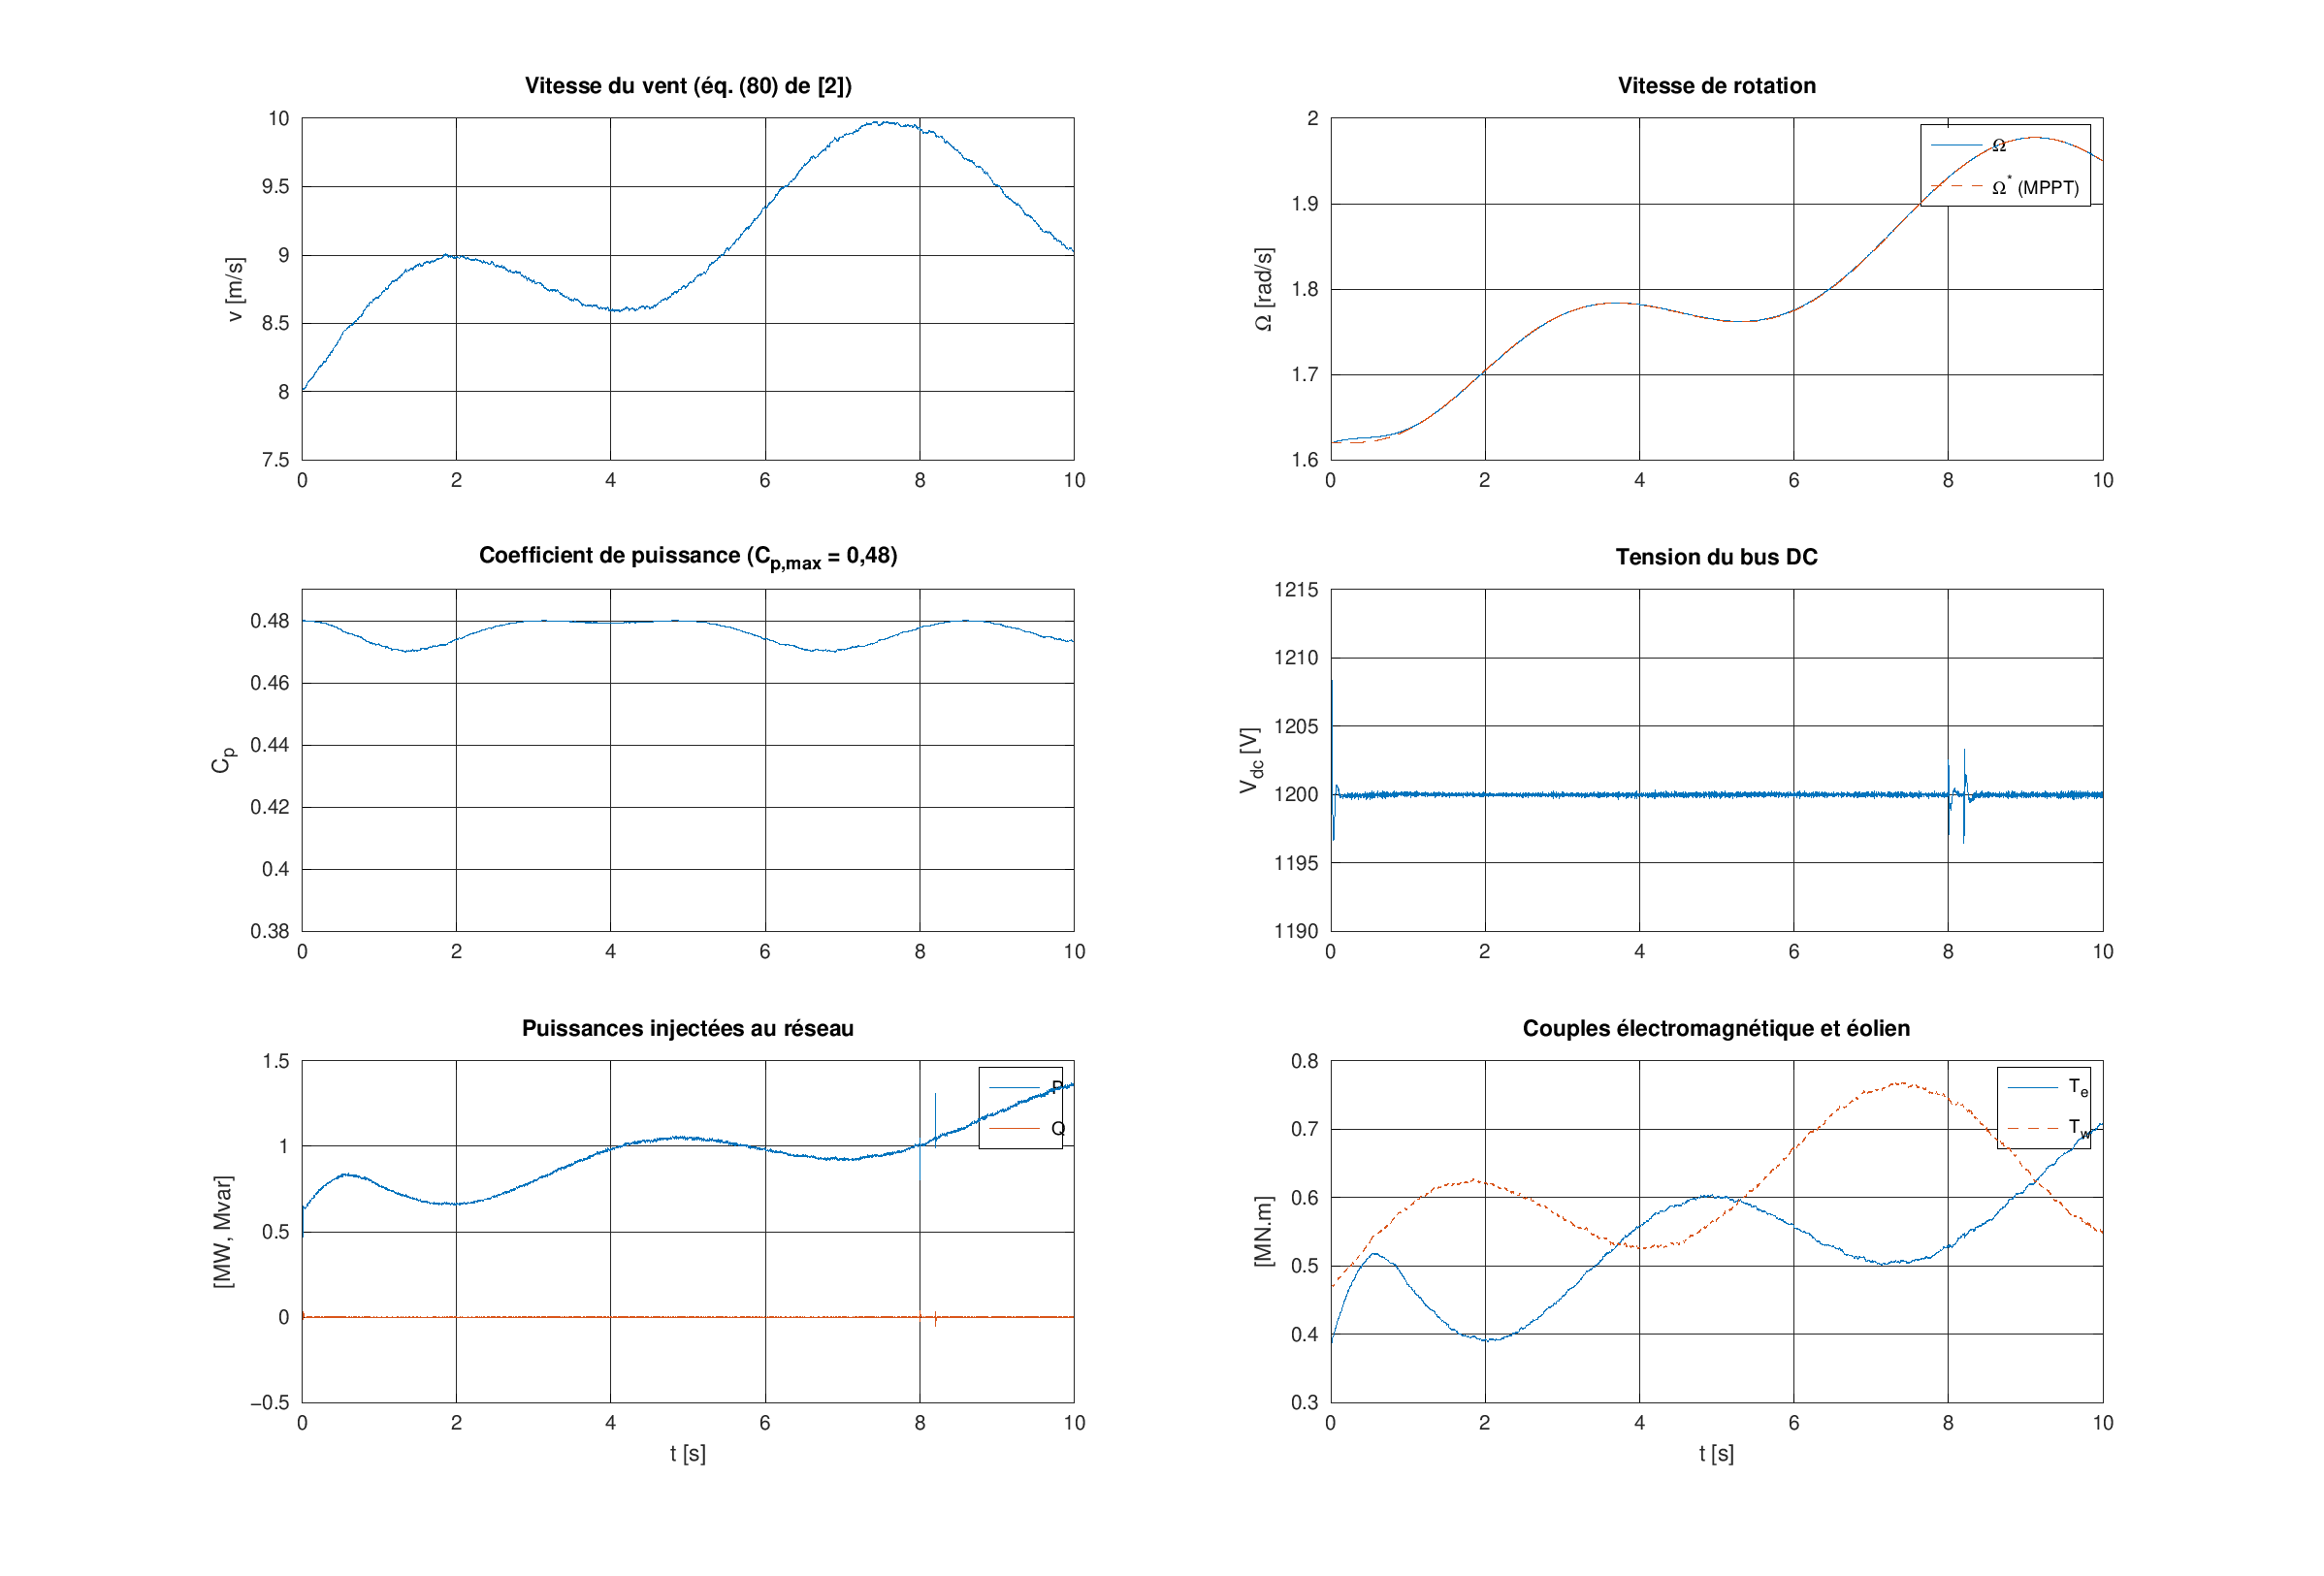
\includegraphics[width=\textwidth]{fig_ensemble.png}
  \caption{Scénario de robustesse avec ANN : vent, vitesse et référence MPPT, $C_p$, tension du bus,
  puissances injectées, couples.}
  \label{fig:ensemble}
\end{figure}

\begin{figure}[h]
  \centering
  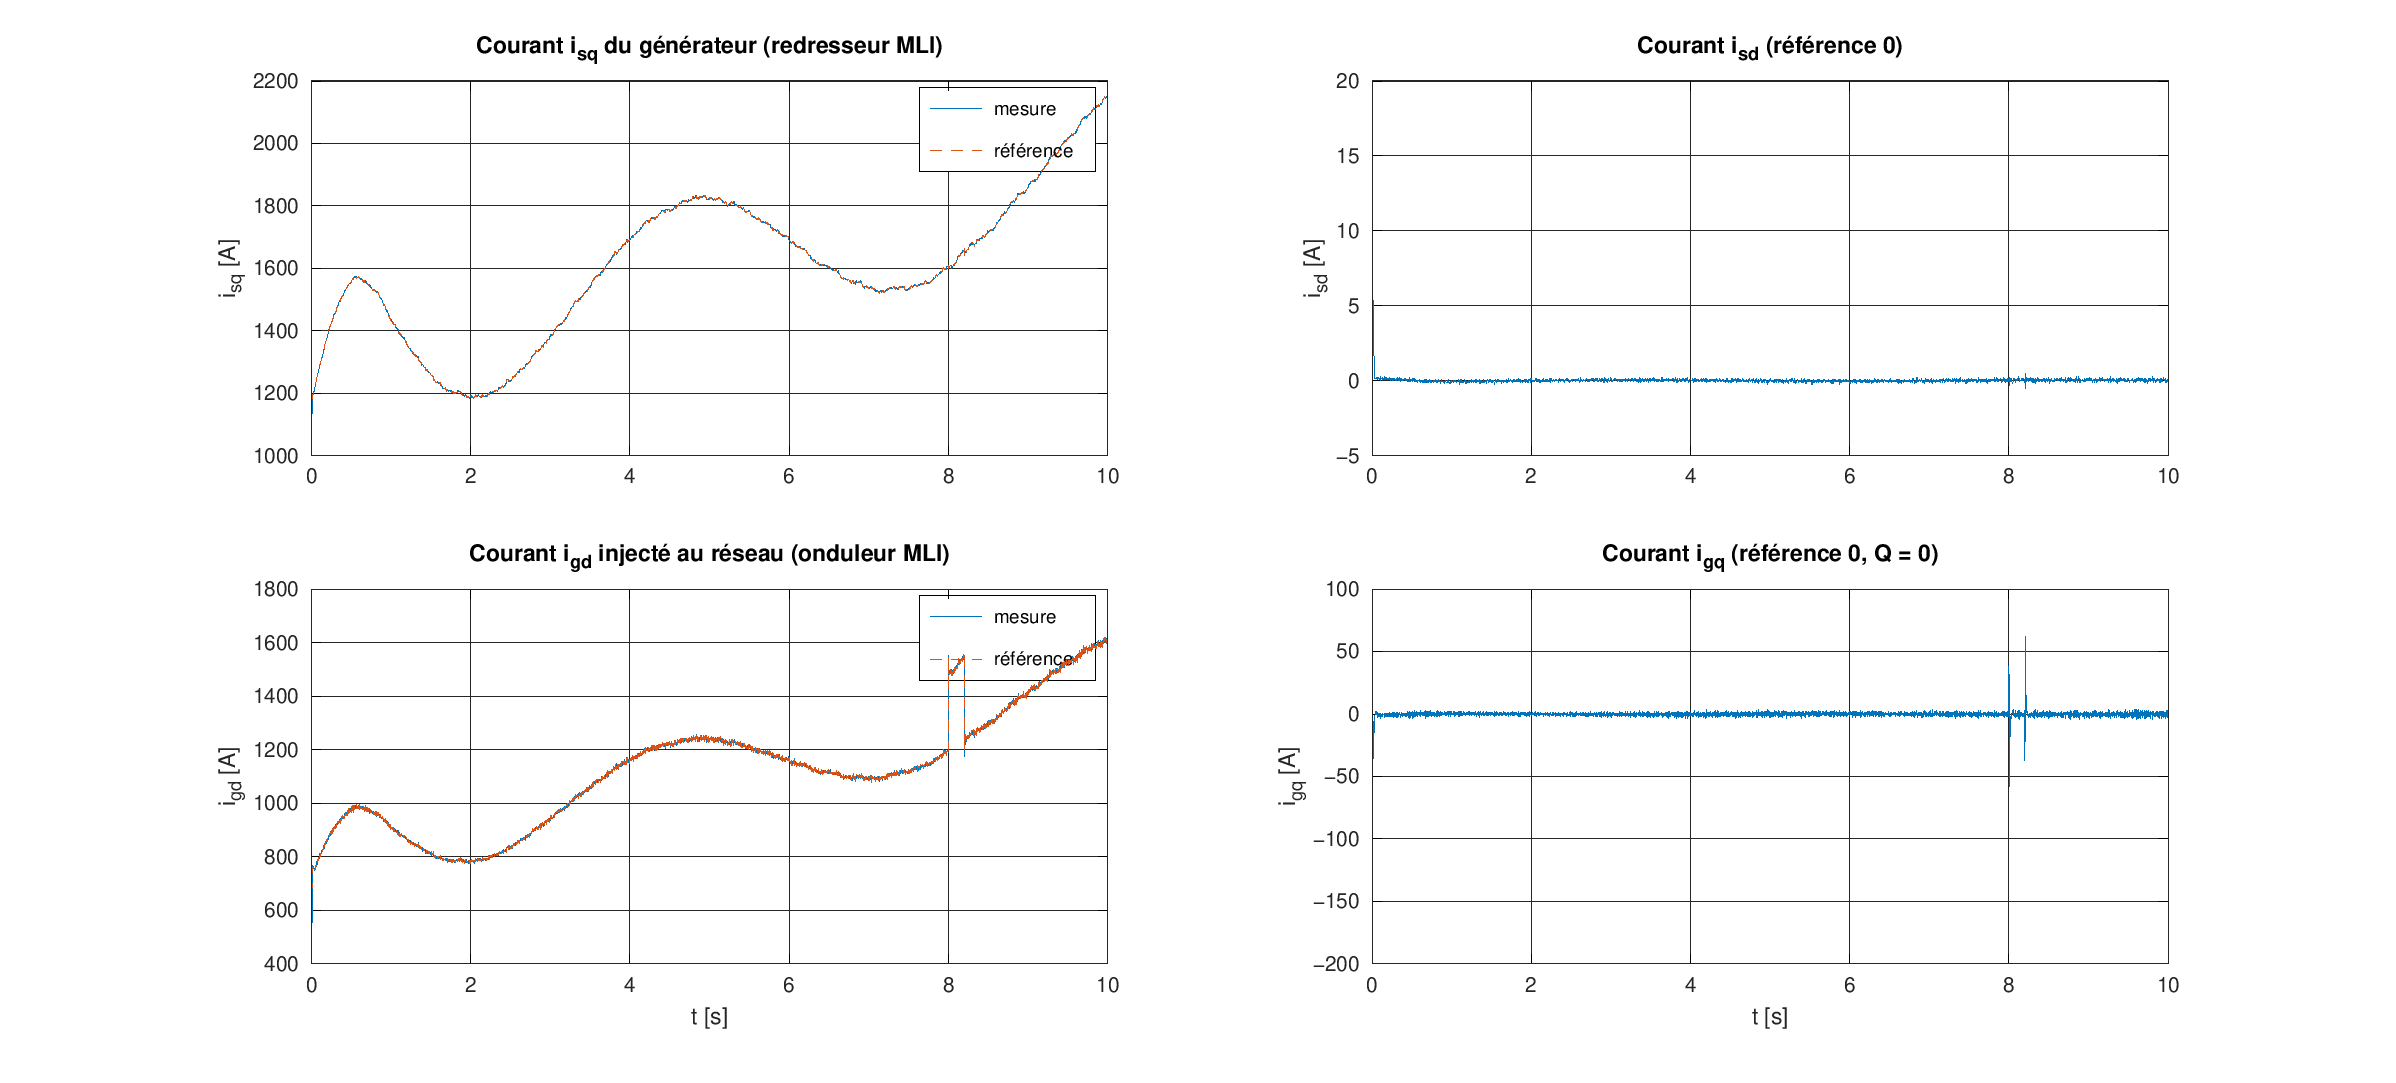
\includegraphics[width=\textwidth]{fig_courants.png}
  \caption{Courants du redresseur et de l'onduleur (commande passive).}
\end{figure}

\begin{figure}[h]
  \centering
  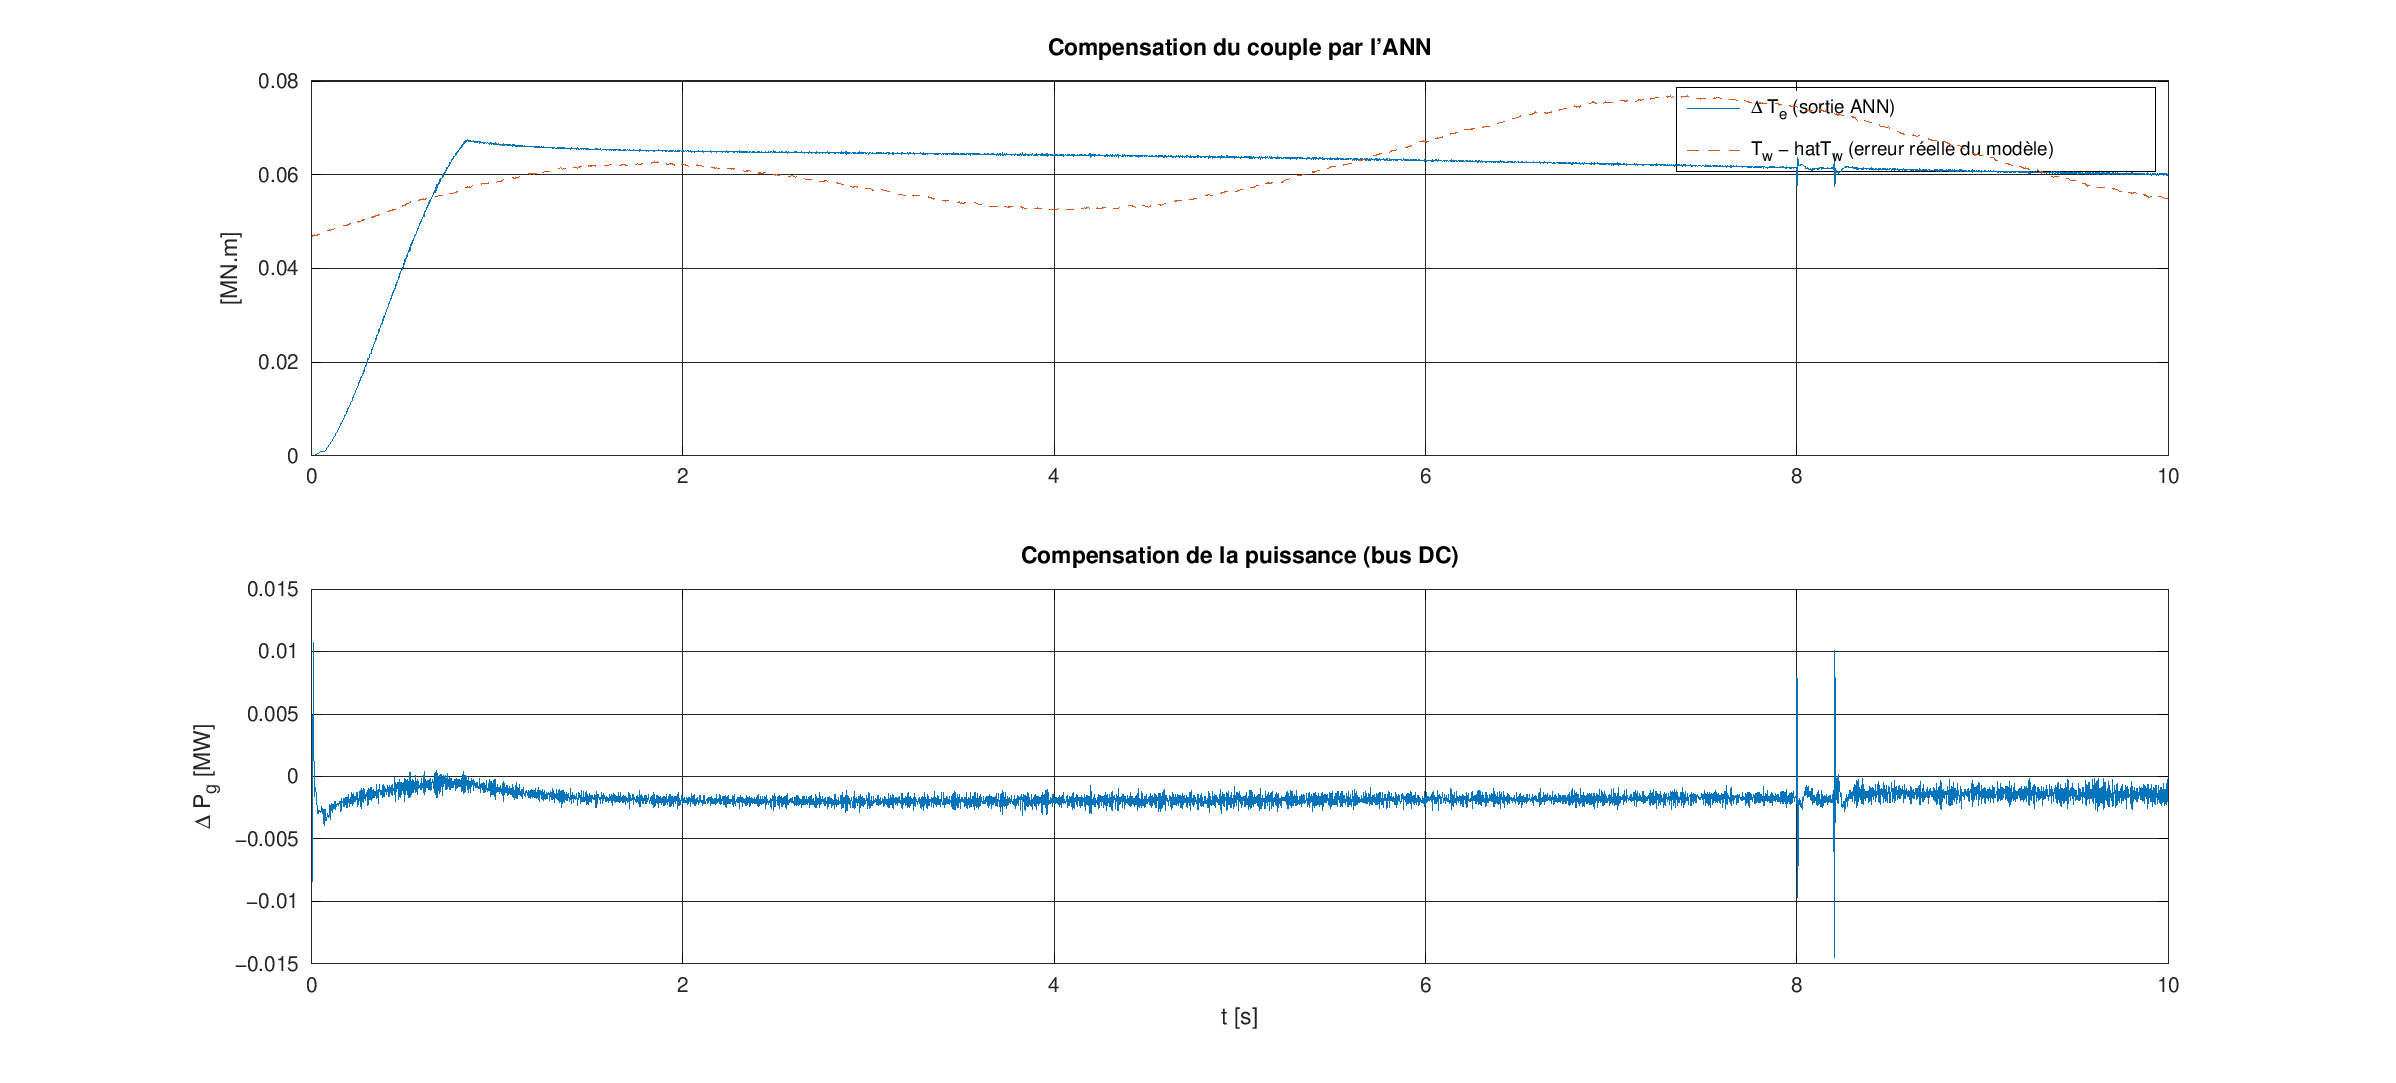
\includegraphics[width=\textwidth]{fig_ann.png}
  \caption{Sortie $\Delta T_e$ de l'ANN comparée à l'erreur réelle du modèle aérodynamique
  $T_w-\hat T_w$ (non connue de l'ANN), et compensation $\Delta P_g$.}
  \label{fig:ann}
\end{figure}

\begin{figure}[h]
  \centering
  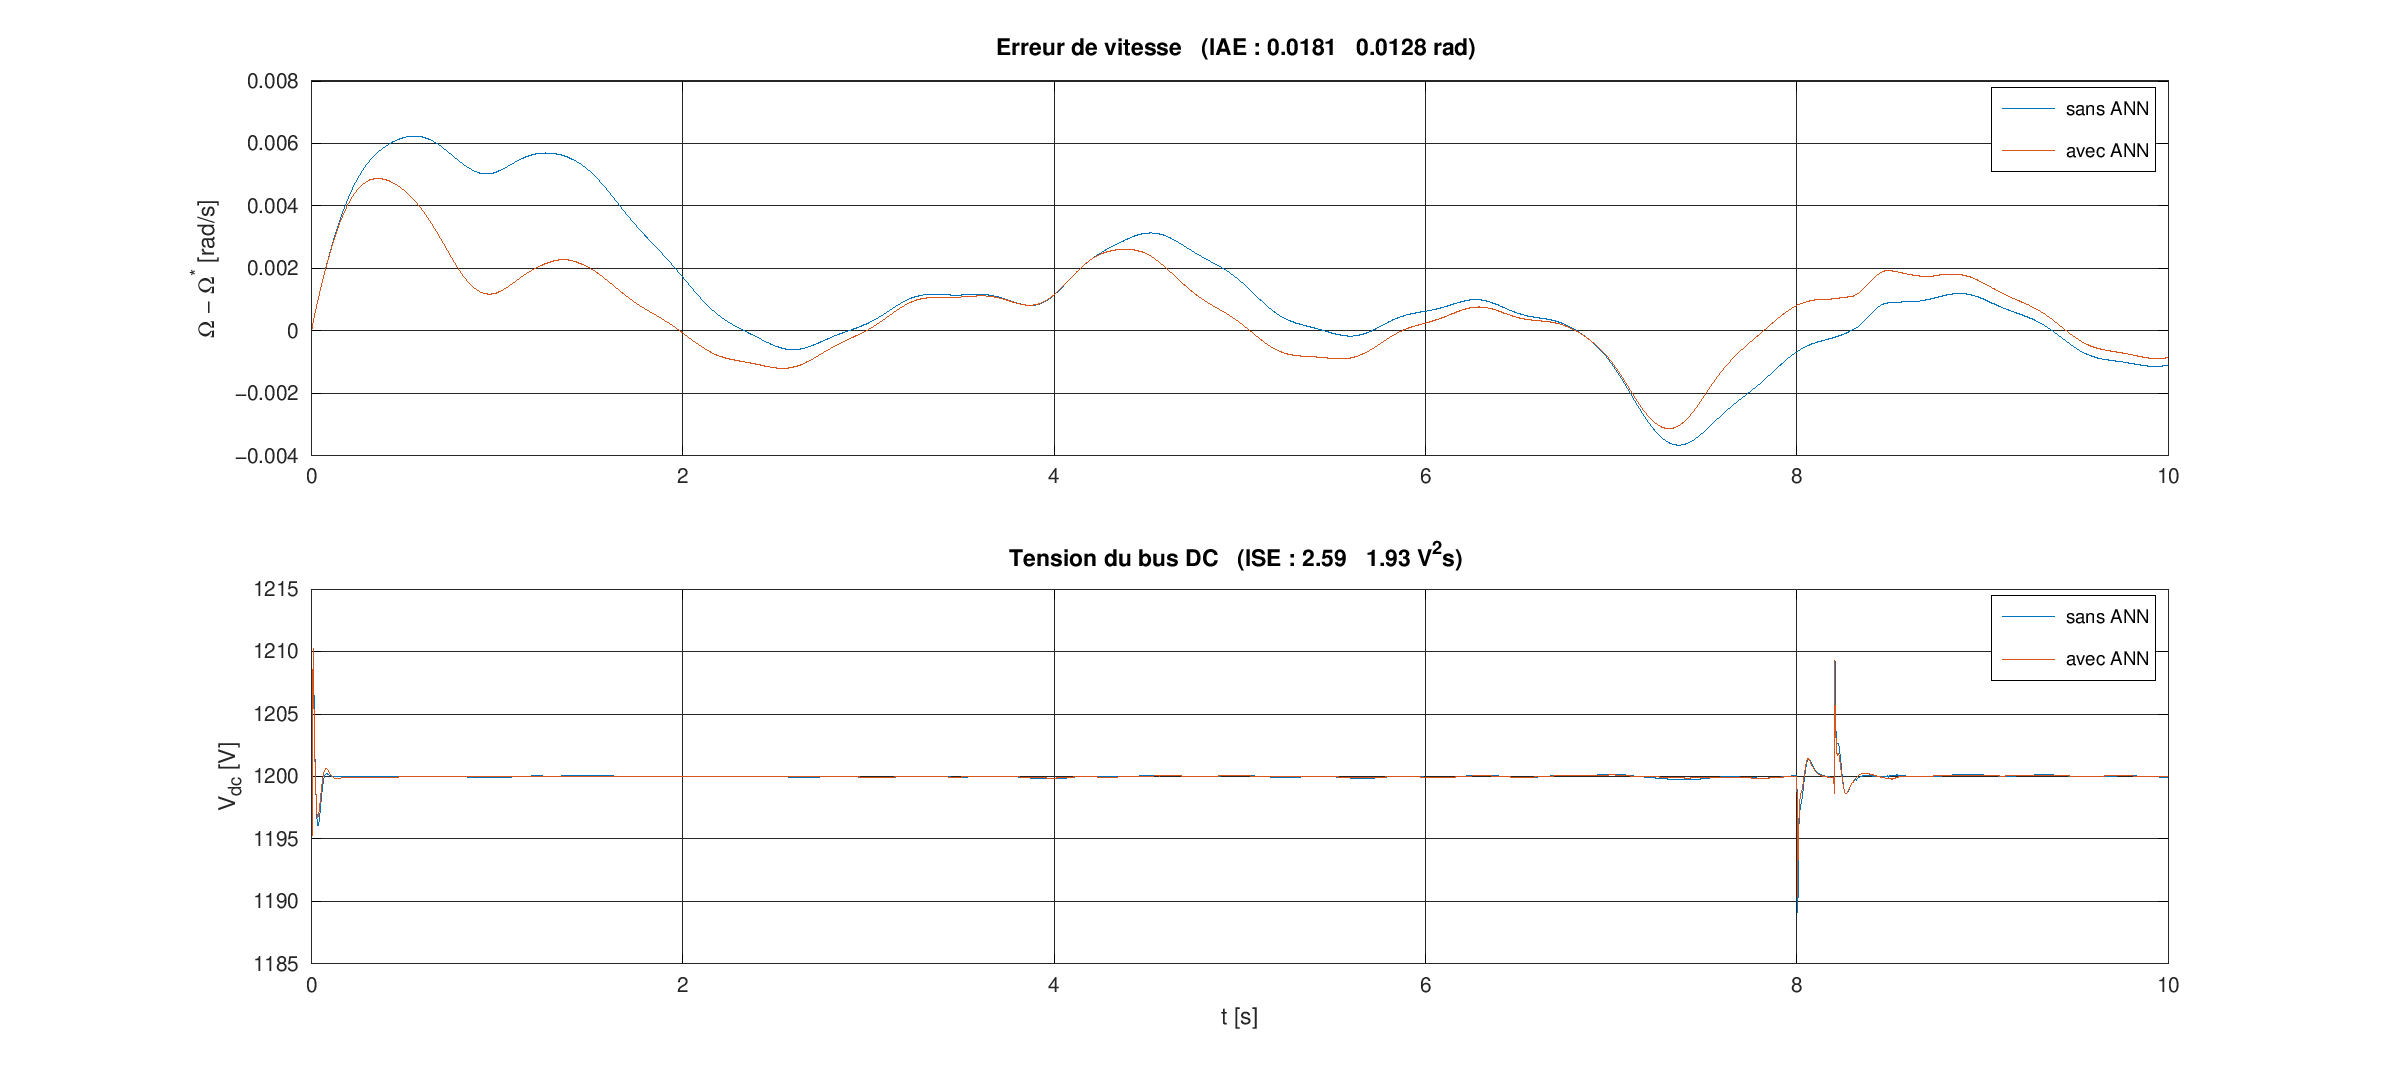
\includegraphics[width=\textwidth]{fig_avec_sans_ann.png}
  \caption{Erreur de vitesse et tension du bus continu, avec et sans ANN (mêmes gains nominaux).}
  \label{fig:comp}
\end{figure}

\clearpage
\subsection{Analyse}
\begin{itemize}
  \item \textbf{Cas nominal.} Les erreurs restent dans la zone morte : l'ANN n'apprend pas et les
        deux commandes sont identiques. La tension du bus reste à $\pm\SI{0,4}{V}$ de
        \SI{1200}{V}, grâce à l'anticipation de $P_{msc}$ dans la loi plate, et $C_p$ reste entre
        0,47 et 0,48.
  \item \textbf{Robustesse.} Avec les mêmes gains, l'ANN réduit l'erreur de vitesse de 39\,\% et
        l'ISE de la tension du bus de 11\,\%. L'écart maximal de la tension du bus (\SI{10,4}{V})
        apparaît au démarrage ($t<\SI{1}{s}$), quand la commande démarre avec des paramètres faux.
        Pendant le creux de tension, l'écart est d'environ \SI{3,5}{V} et la tension revient à
        \SI{1}{V} de sa référence en moins de \SI{40}{ms}.
  \item \textbf{Interprétation de l'ANN} (figure~\ref{fig:ann}). Le modèle $C_p$ de la commande
        sous-estime $T_w$ de 10\,\%. Sans connaître cette erreur, l'ANN converge en moins d'une seconde
        vers $\Delta T_e\approx\SI{0,065}{MN.m}$, soit la valeur moyenne de l'écart réel
        $T_w-\hat T_w$ (entre 0,05 et \SI{0,077}{MN.m}). La partie lentement variable de l'écart est
        prise en charge par l'action intégrale de la loi plate.
  \item \textbf{Énergie.} Le $C_p$ moyen et l'énergie injectée sont pratiquement identiques : le
        gain porte sur la précision du suivi et sur la qualité de la régulation, pas sur l'énergie
        produite.
\end{itemize}

% =====================================================================
\section{Conclusion et limites}
% =====================================================================
La chaîne PMSG \SI{2}{MW} complète a été modélisée (turbine, arbre, PMSG, convertisseurs MLI, bus
continu, filtre $L$, réseau) sous la forme d'un système non linéaire d'ordre 6. La commande associe
la platitude (vitesse et énergie du bus), la passivité (courants des deux convertisseurs) et une
compensation adaptative par réseau de neurones 6-10-2. La stabilité de la commande nominale est
démontrée par une fonction de stockage, et l'erreur reste uniformément ultimement bornée avec l'ANN.

Limites à mentionner :
\begin{itemize}
  \item $J$, $B$ et $R_f$ ne sont pas donnés dans~\cite{hasan} : ce sont des hypothèses ;
  \item pas de commande de l'angle de calage : le vent reste inférieur au vent nominal ;
  \item PLL supposée idéale ; résultats principaux obtenus avec le modèle moyen ;
  \item la loi plate de vitesse utilise le vent mesuré (anémomètre) ;
  \item le gain d'adaptation de l'ANN doit rester modéré ($\Gamma<20$).
\end{itemize}

\begin{thebibliography}{9}
\bibitem{hasan} S.~M.~M. Hasan, A.~H.~M. Shatil, \og Design and Comparison of Grid Connected
Permanent Magnet Synchronous Generator Non-salient Pole and Salient Pole Rotor Wind Turbine \fg,
\emph{AIUB Journal of Science and Engineering (AJSE)}, vol.~20, n°~2, pp.~40--46, 2021.
\bibitem{regani} S.~Regani, M.~Messadi, K.~Kemih, \og A Novel Chaos Control Approach with Adaptive
ANN Compensation for a DFIG-Based Wind Turbine \fg, \emph{Mathematics}, soumis.
\end{thebibliography}

\end{document}
